% effect of temperature on contrastive learning loss function & embedding space

The parameter $\tau$ is called temperature.
\citet{CL_temp_2021} have carried out an exhaustive study on the impact of temperature on the loss function of \ac{cl}.
They found that the contrastive loss function optimizes hard samples by penalizing them according to their hardness.
Small temperatures $\tau$ penalize very hard negative samples, i.e. similar to the anchor.
Hence, the samples' representations are pushed further apart and thus, the embedding space becomes more uniformly distributed \citet{CL_temp_2021,grape_2024}.
However, when $\tau$ is too small, the embedding spaces' semantic structure deteriorates.
For $\tau \rightarrow \infty$, the loss function's hardness-aware property disappears and hard negatives are not penalized anymore.


\begin{figure}%
    \centering
    \subfloat[\centering For small values of $\tau$, similar samples, i.e. x-axis values close to $1.0$, receive high penalties.
    If $\tau$ is too small, only the closest one or two points are penalized and thus, the performance deteriorates.
    As $\tau \rightarrow 1$, the magnitude of the penalty is similar for all negative samples.]
    {{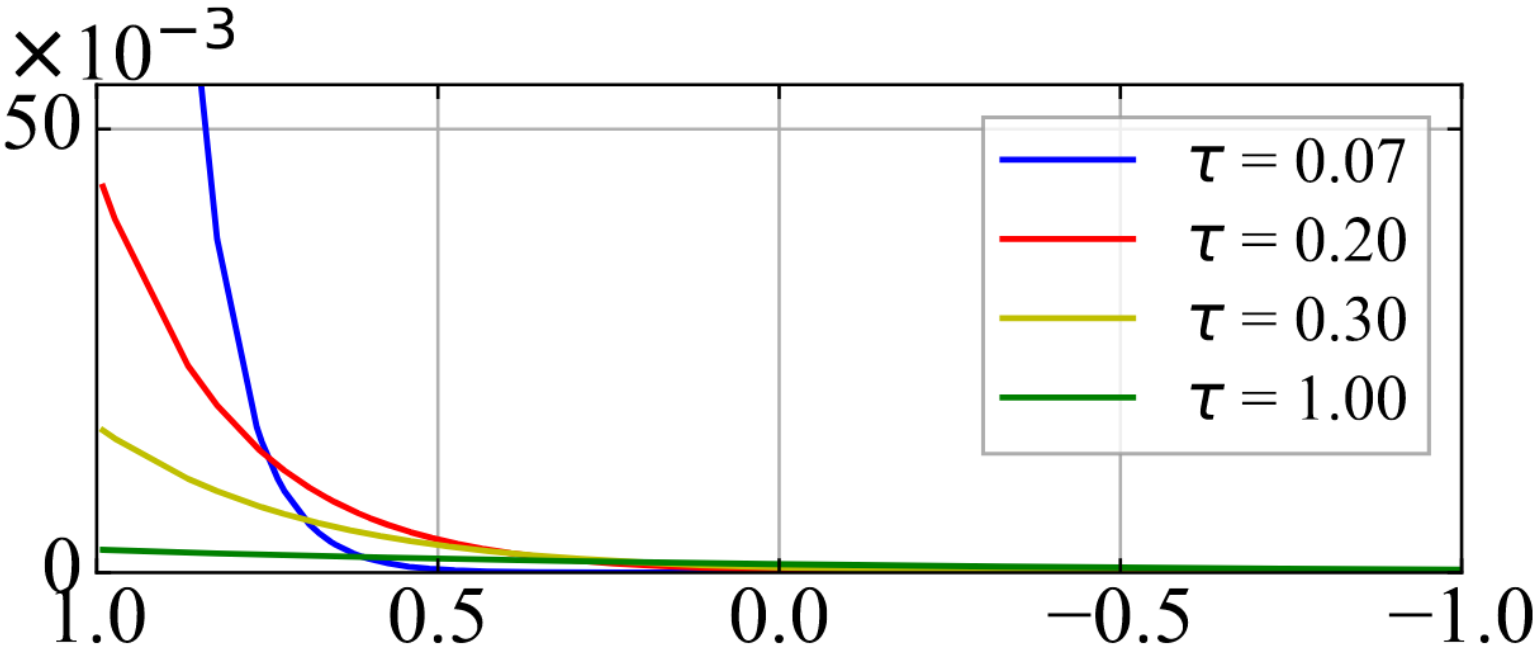
\includegraphics[width=6cm]{images/gradient_ratio_dep_on_temperature.png} }}%
    \qquad
    \subfloat[\centering Visualization of embedding space for different $\tau$.
    Small values of $\tau$ lead to a more uniform distribution of the embedding space, 
    because similar samples are repelled.]
    {{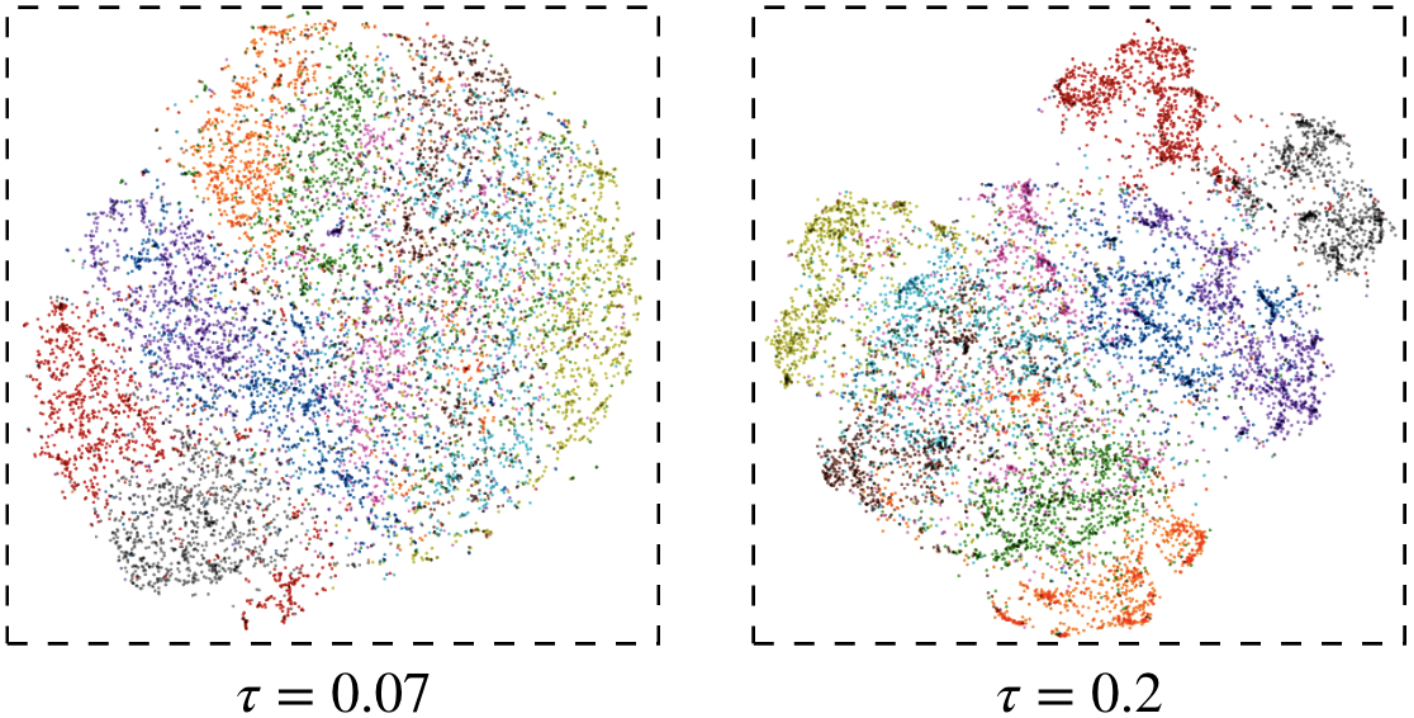
\includegraphics[width=4cm]{images/tsne_dep_on_temperature.png} }}%
    \caption{Illustrations from \citet{CL_temp_2021}.}%
    \label{fig:temperature}%
\end{figure}

% \begin{figure}[h] % h = here, t = top, b = bottom, p = page of floats
%     \centering
%     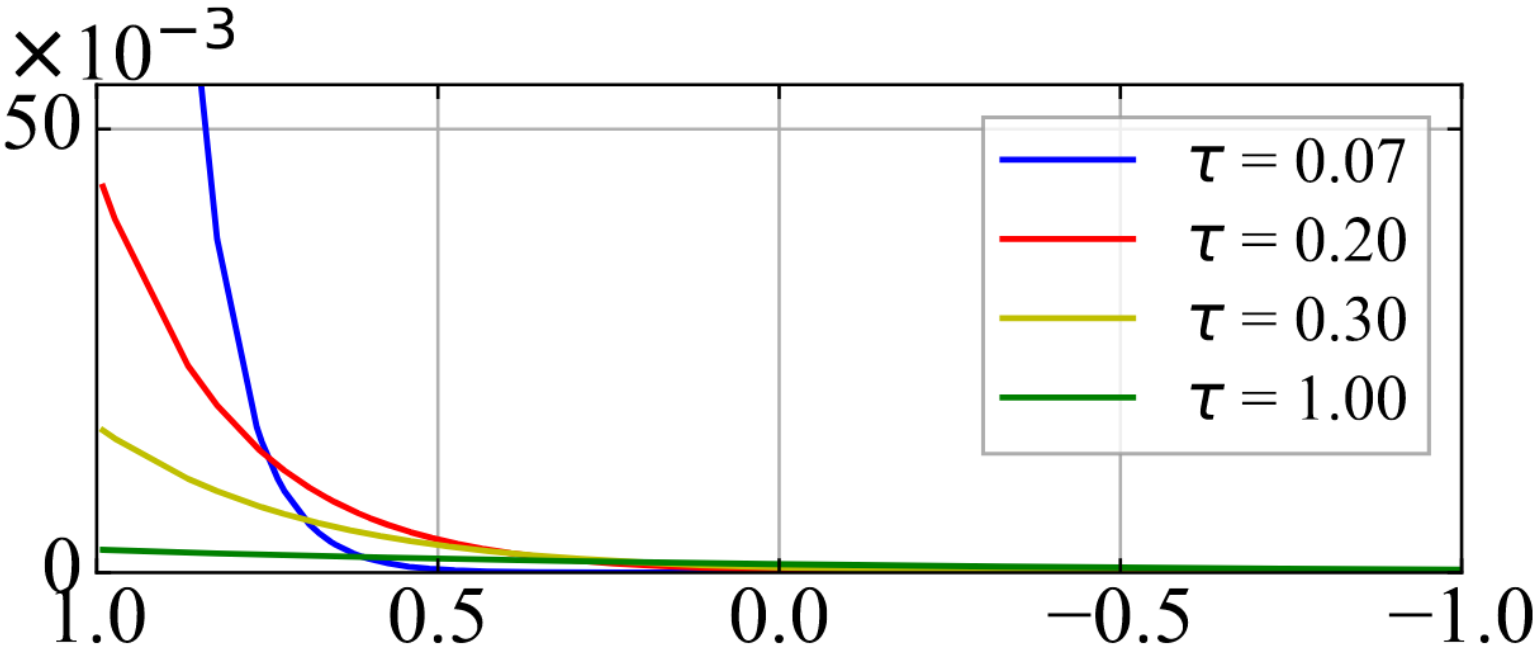
\includegraphics[width=360pt]{images/gradient_ratio_dep_on_temperature.png}
%     \caption{Illustration from \citet{CL_temp_2021}.
%     For small values of $\tau$, similar samples, i.e. x-axis values close to $1.0$, receive high penalties.
%     If $\tau$ is too small, only the closest one or two points are penalized and thus, the performance deteriorates.
%     As $\tau \rightarrow 1$, the magnitude of penalty is similar for all negative samples.
%     }
%     \label{fig:gradient_ratio_dep_on_temperature}
% \end{figure}

% \begin{figure}[h] % h = here, t = top, b = bottom, p = page of floats
%     \centering
%     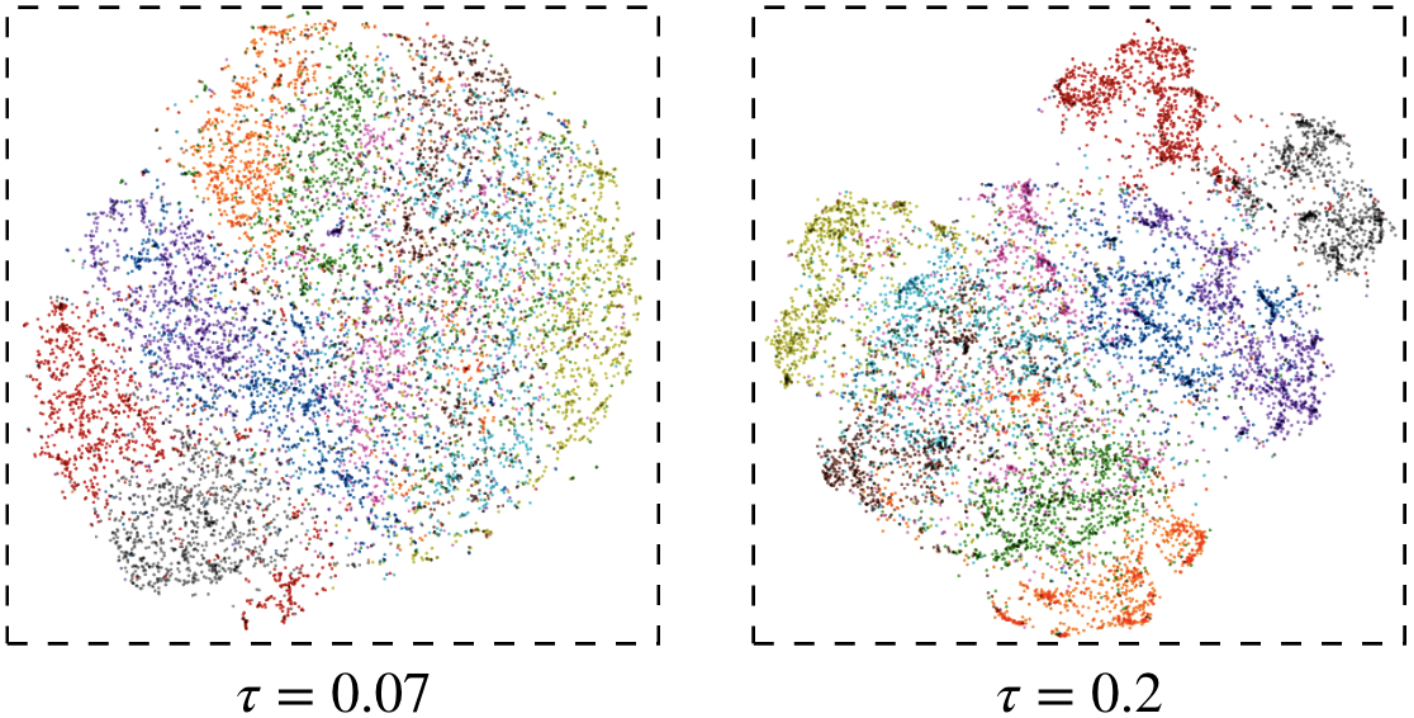
\includegraphics[width=360pt]{images/tsne_dep_on_temperature.png}
%     \caption{Visualization of embedding space for different $\tau$ from \citet{CL_temp_2021}.
%     Small values of $\tau$ lead to a more uniform distribution of the embedding space, 
%     because similar samples are repelled.
%     }
%     \label{fig:tsne_dep_on_temperature}
% \end{figure}

% graph models
% \citet{grape_2024} have worked on a \ac{cl} approach on graphs called \ac{grape}.
% According to \citeauthor{grape_2024}, small values of $\tau$ lead to strong repulsive forces on neighbouring samples.
% Larger values of $\tau$, on the other hand, exert weaker repulse forces.